\documentclass[11pt]{article}
\usepackage[T1]{fontenc}
\usepackage{amsmath,amssymb}
\usepackage{mathrsfs}
\usepackage[margin=1in]{geometry}
\usepackage{microtype}
\usepackage{tikz}
\usetikzlibrary{
  arrows.meta,
  positioning,
  calc,
  fit,
  backgrounds,
  shapes.symbols,
  shapes.geometric
}

\begin{document}

\section{Theoretical Framework}

\subsection{Signal model and scope}
We consider compression of sampled power spectral density (PSD) frames. At each discrete time instant
$t$, a sensing node computes a PSD estimate over a monitored frequency band
$\Omega = [\omega_{\min},\omega_{\max}]$ and must transmit a compact representation to a remote
server under a bitrate constraint.

Let $\{\omega_n\}_{n=1}^{N}$ denote a uniform frequency grid over $\Omega$, and define the sampled
PSD frame
\begin{equation}
\mathbf{s}_t
\triangleq
\begin{bmatrix}
s_{t,1} & \cdots & s_{t,N}
\end{bmatrix}^{\top}
\in \mathbb{R}_{+}^{N},
\qquad
s_{t,n} \triangleq S_t(\omega_n).
\end{equation}
The cloud reconstructs
\begin{equation}
\hat{\mathbf{s}}_t
\triangleq
\begin{bmatrix}
\hat{s}_{t,1} & \cdots & \hat{s}_{t,N}
\end{bmatrix}^{\top}
\in \mathbb{R}_{+}^{N}.
\end{equation}

The framework is composed of three parts:
\begin{enumerate}
    \item a deterministic preprocessing transform with explicit side information,
    \item a learned discrete latent codec with an operational rate model, and
    \item a distortion design consisting of a core PSD fidelity term and an optional task regularizer.
\end{enumerate}

\subsection{Deterministic preprocessing and explicit side information}
To separate deterministic simplification from learned compression, we define the preprocessing map
\begin{equation}
\mathbf{u}_t
=
\mathcal{T}_{\phi_p}(\mathbf{s}_t;\boldsymbol{\tau}_t)
=
\mathcal{S}_{\boldsymbol{\tau}_t}
\!\left(
\Psi_{\kappa}\!\left(
\mathcal{D}_{r}(\mathbf{s}_t)
\right)
\right),
\end{equation}
where:
\begin{itemize}
    \item $r \in (0,1]$ is a frequency-resolution factor,
    \item $\mathcal{D}_{r} : \mathbb{R}_{+}^{N} \to \mathbb{R}_{+}^{N_r}$ is a deterministic
    downsampling operator with
    \begin{equation}
    N_r \triangleq \lfloor rN \rfloor,
    \end{equation}
    \item $\Psi_{\kappa} : \mathbb{R}_{+}^{N_r} \to \mathbb{R}^{N_r}$ is an elementwise
    dynamic-range map,
    \item $\mathcal{S}_{\boldsymbol{\tau}_t} : \mathbb{R}^{N_r} \to \mathbb{R}^{N_r}$ is a
    blockwise standardization operator parameterized by frame-dependent side information
    $\boldsymbol{\tau}_t$,
    \item $\phi_p$ collects the fixed preprocessing hyperparameters.
\end{itemize}

\paragraph{Admissible preprocessing operators.}
The operators $\mathcal{D}_{r}$ and $\mathcal{U}_{r}$ are assumed to be fixed and deterministic,
with
\begin{equation}
\mathcal{D}_{r} : \mathbb{R}_{+}^{N} \to \mathbb{R}_{+}^{N_r},
\qquad
\mathcal{U}_{r} : \mathbb{R}_{+}^{N_r} \to \mathbb{R}_{+}^{N},
\end{equation}
and they must satisfy:
\begin{enumerate}
    \item \emph{nonnegativity preservation:}
    \begin{equation}
    \mathcal{D}_{r}(\mathbb{R}_{+}^{N}) \subseteq \mathbb{R}_{+}^{N_r},
    \qquad
    \mathcal{U}_{r}(\mathbb{R}_{+}^{N_r}) \subseteq \mathbb{R}_{+}^{N};
    \end{equation}

    \item \emph{constant-spectrum consistency:} for every $c \ge 0$,
    \begin{equation}
    \mathcal{U}_{r}\!\big(\mathcal{D}_{r}(c\mathbf{1}_{N})\big)
    =
    c\mathbf{1}_{N},
    \end{equation}
    where $\mathbf{1}_{N}$ denotes the all-ones vector in $\mathbb{R}^{N}$;

    \item \emph{boundedness:} there exist finite constants $C_D, C_U > 0$ such that
    \begin{equation}
    \|\mathcal{D}_{r}(\mathbf{x})\|_2 \le C_D\|\mathbf{x}\|_2,
    \qquad
    \|\mathcal{U}_{r}(\mathbf{y})\|_2 \le C_U\|\mathbf{y}\|_2
    \end{equation}
    for all $\mathbf{x} \in \mathbb{R}_{+}^{N}$ and $\mathbf{y} \in \mathbb{R}_{+}^{N_r}$.
\end{enumerate}
A concrete admissible default is local block averaging for $\mathcal{D}_{r}$ and linear
interpolation for $\mathcal{U}_{r}$, but the framework itself only requires the properties above.

\paragraph{Dynamic-range mapping.}
Let
\begin{equation}
\mathbf{x}_t
\triangleq
\Psi_{\kappa}\!\left(\mathcal{D}_{r}(\mathbf{s}_t)\right),
\qquad
[\Psi_{\kappa}(\mathbf{v})]_n = \log(v_n + \kappa),
\qquad
\kappa > 0.
\end{equation}
Its inverse is applied elementwise as
\begin{equation}
[\Psi_{\kappa}^{-1}(\mathbf{x})]_n = e^{x_n} - \kappa.
\end{equation}
This fixes the nonlinearity explicitly while preserving invertibility.

\paragraph{Blockwise standardization.}
Partition the reduced grid into $B$ contiguous blocks
$\{\mathcal{B}_b\}_{b=1}^{B}$, and let $b(n)$ denote the block containing bin $n$.
For each block, define
\begin{align}
\mu_{t,b}
&\triangleq
\frac{1}{|\mathcal{B}_b|}
\sum_{n \in \mathcal{B}_b} x_{t,n}, \\
\sigma_{t,b}
&\triangleq
\left(
\frac{1}{|\mathcal{B}_b|}
\sum_{n \in \mathcal{B}_b}
(x_{t,n}-\mu_{t,b})^2
+
\varepsilon_{\sigma}
\right)^{1/2},
\qquad
\varepsilon_{\sigma} > 0.
\end{align}
The standardized representation is
\begin{equation}
u_{t,n}
=
\frac{x_{t,n}-\mu_{t,b(n)}}{\sigma_{t,b(n)}},
\qquad
\mathbf{u}_t
\triangleq
\begin{bmatrix}
u_{t,1} & \cdots & u_{t,N_r}
\end{bmatrix}^{\top}.
\end{equation}

The side-information vector is
\begin{equation}
\boldsymbol{\tau}_t
\triangleq
\begin{bmatrix}
\mu_{t,1} &
\log \sigma_{t,1} &
\cdots &
\mu_{t,B} &
\log \sigma_{t,B}
\end{bmatrix}^{\top}.
\end{equation}
We quantize $\boldsymbol{\tau}_t$ to $\hat{\boldsymbol{\tau}}_t$ using fixed scalar quantizers.
If $q_{\mu}$ bits are used for each $\mu_{t,b}$ and $q_{\sigma}$ bits for each $\log \sigma_{t,b}$,
then the side-information rate is
\begin{equation}
L_{\tau}^{(t)} \triangleq B(q_{\mu}+q_{\sigma}).
\end{equation}
This cost is charged explicitly and is not treated as negligible overhead.

\paragraph{Inverse preprocessing.}
The inverse standardization operator
$\mathcal{S}_{\hat{\boldsymbol{\tau}}_t}^{-1} : \mathbb{R}^{N_r} \to \mathbb{R}^{N_r}$
is defined componentwise by
\begin{equation}
\left[
\mathcal{S}_{\hat{\boldsymbol{\tau}}_t}^{-1}(\mathbf{u})
\right]_n
=
\hat{\sigma}_{t,b(n)}u_n + \hat{\mu}_{t,b(n)}.
\end{equation}
Accordingly, the inverse preprocessing chain is
\begin{equation}
\mathcal{T}_{\phi_p}^{-1}(\mathbf{u};\hat{\boldsymbol{\tau}}_t)
=
\mathcal{U}_{r}
\!\left(
\Psi_{\kappa}^{-1}
\!\left(
\mathcal{S}_{\hat{\boldsymbol{\tau}}_t}^{-1}(\mathbf{u})
\right)
\right).
\end{equation}

\begin{figure}[t]
\centering
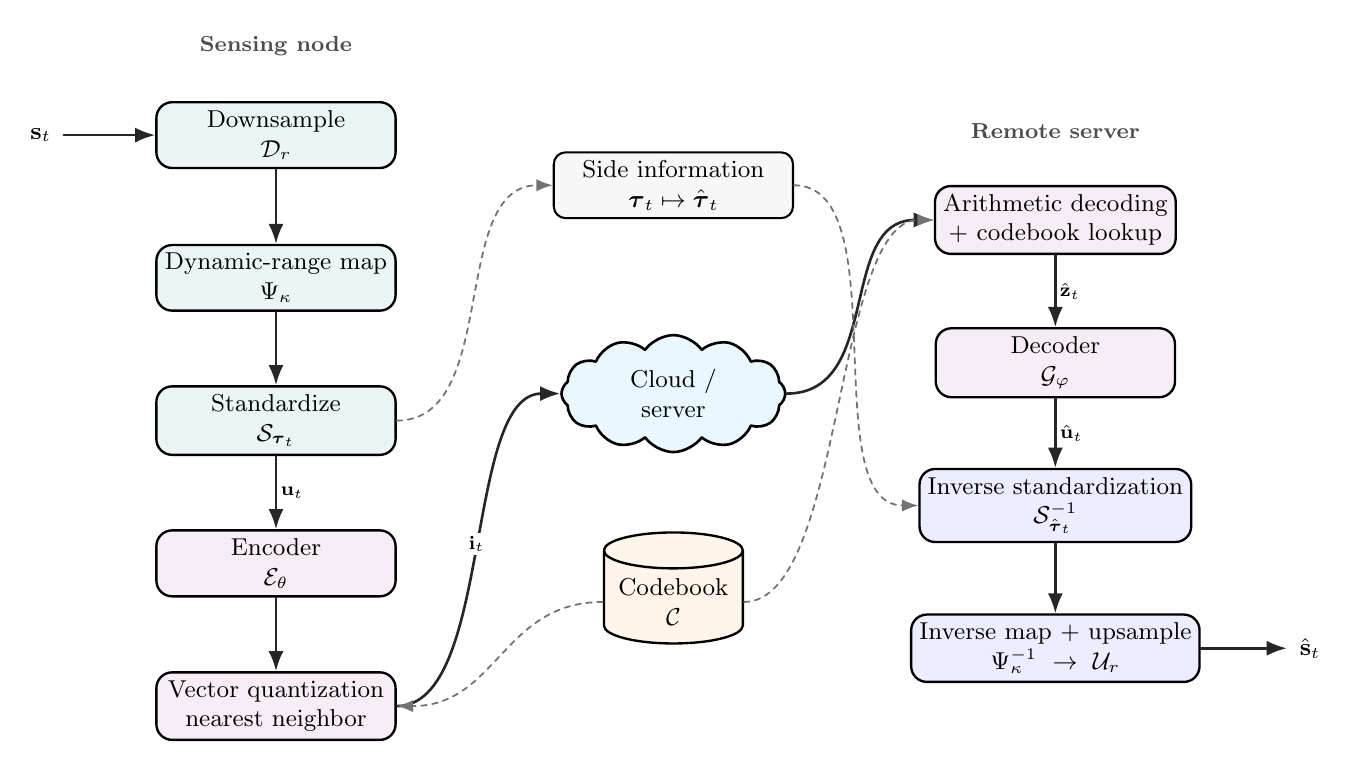
\begin{tikzpicture}[
  x=1cm, y=1cm,
  >={Latex[length=2.6mm,width=1.9mm]},
  scale=0.98,
  transform shape,
  font=\small,
  line cap=round,
  line join=round,
  flow/.style={
    -Latex,
    line width=0.95pt,
    draw=black!85
  },
  aux/.style={
    -Latex,
    line width=0.65pt,
    draw=black!55,
    dash pattern=on 2pt off 2pt
  },
  proc/.style={
    draw,
    rounded corners=2mm,
    line width=0.85pt,
    fill=teal!8,
    minimum width=31mm,
    minimum height=8.5mm,
    align=center,
    inner sep=3pt
  },
  codec/.style={
    draw,
    rounded corners=2mm,
    line width=0.85pt,
    fill=violet!7,
    minimum width=31mm,
    minimum height=8.5mm,
    align=center,
    inner sep=3pt
  },
  recon/.style={
    draw,
    rounded corners=2mm,
    line width=0.85pt,
    fill=blue!7,
    minimum width=31mm,
    minimum height=8.5mm,
    align=center,
    inner sep=3pt
  },
  cloudnode/.style={
    draw,
    cloud,
    cloud puffs=12,
    cloud puff arc=110,
    aspect=2.1,
    minimum width=29mm,
    minimum height=14mm,
    fill=cyan!9,
    line width=0.95pt,
    align=center
  },
  db/.style={
    draw,
    cylinder,
    shape border rotate=90,
    aspect=0.28,
    minimum height=11mm,
    minimum width=18mm,
    fill=orange!8,
    line width=0.85pt,
    align=center
  },
  sidenote/.style={
    draw,
    rounded corners=1.5mm,
    fill=gray!6,
    line width=0.75pt,
    minimum width=31mm,
    minimum height=8mm,
    align=center,
    inner sep=3pt
  },
  io/.style={
    align=center,
    inner sep=1pt
  },
  lab/.style={
    font=\scriptsize,
    fill=white,
    inner sep=1.2pt,
    text=black
  }
]

% Main nodes
\node[proc]  (dr)   at (-4.85,  2.20) {Downsample\\$\mathcal{D}_r$};
\node[proc]  (psi)  at (-4.85,  0.35) {Dynamic-range map\\$\Psi_\kappa$};
\node[proc]  (std)  at (-4.85, -1.50) {Standardize\\$\mathcal{S}_{\boldsymbol{\tau}_t}$};
\node[codec] (enc)  at (-4.85, -3.35) {Encoder\\$\mathcal{E}_\theta$};
\node[codec] (vq)   at (-4.85, -5.20) {Vector quantization\\nearest neighbor};

% Center column
\node[sidenote]  (side)  at (0.30,  1.55)
  {Side information\\$\boldsymbol{\tau}_t \mapsto \hat{\boldsymbol{\tau}}_t$};

\node[cloudnode] (cloud) at (0.30, -1.15) {Cloud /\\server};

\node[db]        (cb)    at (0.30, -3.85) {Codebook\\$\mathcal{C}$};

% Remote server
\node[codec] (ad)   at (5.25,  1.10) {Arithmetic decoding\\+ codebook lookup};
\node[codec] (dec)  at (5.25, -0.75) {Decoder\\$\mathcal{G}_\varphi$};
\node[recon] (istd) at (5.25, -2.60) {Inverse standardization\\$\mathcal{S}^{-1}_{\hat{\boldsymbol{\tau}}_t}$};
\node[recon] (iup)  at (5.25, -4.45) {Inverse map + upsample\\$\Psi_\kappa^{-1}\ \rightarrow\ \mathcal{U}_r$};

% External I/O
\coordinate (sin)  at (-7.60,  2.20);
\coordinate (sout) at ( 8.25, -4.45);

\node[io] at (-7.90,  2.20) {$\mathbf{s}_t$};
\node[io] at ( 8.55, -4.45) {$\hat{\mathbf{s}}_t$};

% Main flow
\draw[flow] (sin) -- (dr.west);

\draw[flow] (dr.south)   -- (psi.north);
\draw[flow] (psi.south)  -- (std.north);
\draw[flow] (std.south)  -- node[midway,right,lab] {$\mathbf{u}_t$} (enc.north);
\draw[flow] (enc.south)  -- (vq.north);

\draw[flow]
  (vq.east)
  .. controls +(1.25,0) and +(-1.25,0) ..
  node[lab, above=1pt, pos=0.48] {$\mathbf{i}_t$}
  (cloud.west);

\draw[flow]
  (cloud.east)
  .. controls +(1.25,0) and +(-1.25,0) ..
  (ad.west);

\draw[flow] (ad.south)   -- node[midway,right,lab] {$\hat{\mathbf{z}}_t$} (dec.north);
\draw[flow] (dec.south)  -- node[midway,right,lab] {$\hat{\mathbf{u}}_t$} (istd.north);
\draw[flow] (istd.south) -- (iup.north);
\draw[flow] (iup.east) -- (sout);

% Side-information branch
\draw[aux]
  (std.east)
  .. controls +(1.35,0) and +(-1.35,0) ..
  (side.west);

\draw[aux]
  (side.east)
  .. controls +(1.35,0) and +(-1.35,0) ..
  (istd.west);

% Codebook links
\draw[aux]
  (cb.west)
  .. controls +(-1.30,0) and +(1.30,0) ..
  (vq.east);

\draw[aux]
  (cb.east)
  .. controls +(1.30,0) and +(-1.30,0) ..
  (ad.west);

% Group labels
\node[font=\footnotesize\bfseries, text=black!70] at (-4.85, 3.35) {Sensing node};
\node[font=\footnotesize\bfseries, text=black!70] at (5.25, 2.25) {Remote server};

\end{tikzpicture}
\caption{
End-to-end workflow of the proposed PSD codec. A PSD frame $\mathbf{s}_t$ is deterministically
preprocessed, encoded into discrete indices, transmitted to the cloud/server, and reconstructed as
$\hat{\mathbf{s}}_t$. The side-information path
$\boldsymbol{\tau}_t \mapsto \hat{\boldsymbol{\tau}}_t$ is explicit because its payload contributes
to the bitrate budget through $L_{\tau}^{(t)}$.
}
\label{fig:psdcodec_workflow}
\end{figure}

\subsection{Learned discrete latent codec}
The learned codec acts on the preprocessed frame $\mathbf{u}_t$. Let
\begin{equation}
\mathbf{z}_t
=
\mathcal{E}_{\theta}(\mathbf{u}_t)
=
\begin{bmatrix}
\mathbf{z}_{t,1} & \cdots & \mathbf{z}_{t,M}
\end{bmatrix},
\qquad
\mathbf{z}_{t,m} \in \mathbb{R}^{d},
\end{equation}
where $M$ is the number of latent positions and $d$ is the latent embedding dimension.

Let the codebook be
\begin{equation}
\mathcal{C}
=
\{\mathbf{c}_1,\ldots,\mathbf{c}_J\},
\qquad
\mathbf{c}_j \in \mathbb{R}^{d}.
\end{equation}
Each latent vector is quantized to its nearest codeword:
\begin{align}
i_{t,m}
&\triangleq
\operatorname*{arg\,min}_{1 \le j \le J}
\|\mathbf{z}_{t,m}-\mathbf{c}_j\|_2^2, \\
\hat{\mathbf{z}}_{t,m}
&\triangleq
\mathbf{c}_{i_{t,m}}.
\end{align}
The discrete index sequence is
\begin{equation}
\mathbf{i}_t
\triangleq
\begin{bmatrix}
i_{t,1} & \cdots & i_{t,M}
\end{bmatrix}^{\top},
\end{equation}
and the corresponding quantized latent representation is
\begin{equation}
\hat{\mathbf{z}}_t
\triangleq
\begin{bmatrix}
\hat{\mathbf{z}}_{t,1} & \cdots & \hat{\mathbf{z}}_{t,M}
\end{bmatrix}.
\end{equation}

The decoder reconstructs the normalized representation as
\begin{equation}
\hat{\mathbf{u}}_t
=
\mathcal{G}_{\varphi}(\hat{\mathbf{z}}_t),
\end{equation}
and the final PSD reconstruction is
\begin{equation}
\hat{\mathbf{s}}_t
=
\mathcal{T}_{\phi_p}^{-1}(\hat{\mathbf{u}}_t;\hat{\boldsymbol{\tau}}_t).
\end{equation}

During training, the non-differentiable nearest-neighbor assignment is handled with the
straight-through estimator, and the vector-quantization stabilization loss is
\begin{equation}
\mathcal{L}_{\mathrm{VQ}}^{(t)}
=
\sum_{m=1}^{M}
\left(
\big\|
\operatorname{sg}[\mathbf{z}_{t,m}] - \hat{\mathbf{z}}_{t,m}
\big\|_2^2
+
\beta_{\mathrm{com}}
\big\|
\mathbf{z}_{t,m} - \operatorname{sg}[\hat{\mathbf{z}}_{t,m}]
\big\|_2^2
\right),
\end{equation}
where $\operatorname{sg}[\cdot]$ denotes the stop-gradient operator and
$\beta_{\mathrm{com}} > 0$ is the commitment weight.

\subsection{Operational rate model}
Because the system is a codec rather than merely an autoencoder, the rate term must be modeled
explicitly. Let
\begin{equation}
q_{\xi}(\mathbf{i}_t)
=
\prod_{m=1}^{M}
q_{\xi}(i_{t,m}\mid \mathbf{h}_{t,m}),
\end{equation}
where $q_{\xi}$ is an entropy model and $\mathbf{h}_{t,m}$ denotes optional causal context
(e.g., previously decoded indices or side information derived from a hyperprior). A factorized model
is recovered by taking $\mathbf{h}_{t,m}=\varnothing$.

The differentiable training-time rate proxy for the main index stream is
\begin{equation}
R_{\mathrm{idx}}^{(t)}
\triangleq
-\sum_{m=1}^{M}
\log_{2} q_{\xi}(i_{t,m}\mid \mathbf{h}_{t,m}).
\end{equation}
Including side information, the total training-time rate surrogate is
\begin{equation}
R_{\mathrm{e}}^{(t)}
\triangleq
R_{\mathrm{idx}}^{(t)} + L_{\tau}^{(t)}.
\end{equation}

At deployment, the sequence $\mathbf{i}_t$ is arithmetic-coded under the same model, yielding an
actual coded length $L_{\mathrm{idx},\mathrm{ac}}^{(t)}$. The operational payload is therefore
\begin{equation}
L_{\mathrm{op}}^{(t)}
\triangleq
L_{\mathrm{idx},\mathrm{ac}}^{(t)} + L_{\tau}^{(t)}.
\end{equation}
Reported rate--distortion curves should be based on $L_{\mathrm{op}}^{(t)}$, not merely on
$R_{\mathrm{e}}^{(t)}$.

\subsection{Reference noise floor and occupancy representation}
Occupancy-related quantities depend on a noise-floor baseline, so that baseline must be defined
externally to the codec. Let
\begin{equation}
\bar{\mathbf{n}}_t
\triangleq
\begin{bmatrix}
\bar{n}_{t,1} & \cdots & \bar{n}_{t,N}
\end{bmatrix}^{\top}
\in \mathbb{R}_{+}^{N}
\end{equation}
be a reference noise-floor estimate obtained from uncompressed frames over a sliding window of
length $W$, with
\begin{equation}
\bar{n}_{t,n}
\triangleq
\mathcal{N}\!\left(
\{s_{\tau,n}\}_{\tau=t-W+1}^{t}
\right),
\end{equation}
where $\mathcal{N}$ is a robust baseline estimator (e.g., a lower percentile, trimmed mean, or
calibration-based rule).

To avoid conflating compression error with baseline-estimation error, the same
$\bar{\mathbf{n}}_t$ and threshold margin $\gamma$ are used to define occupancy from both
$\mathbf{s}_t$ and $\hat{\mathbf{s}}_t$ during training and primary evaluation.
For differentiability, define
\begin{equation}
\sigma_{\tau_{\mathrm{occ}}}(x)
=
\frac{1}{1+\exp(-x/\tau_{\mathrm{occ}})},
\qquad
\tau_{\mathrm{occ}} > 0,
\end{equation}
and the soft occupancies
\begin{align}
p_{t,n}
&\triangleq
\sigma_{\tau_{\mathrm{occ}}}(s_{t,n}-\bar{n}_{t,n}-\gamma), \\
\hat{p}_{t,n}
&\triangleq
\sigma_{\tau_{\mathrm{occ}}}(\hat{s}_{t,n}-\bar{n}_{t,n}-\gamma).
\end{align}
Their hard-thresholded versions are
\begin{equation}
o_{t,n} = \mathbf{1}\{p_{t,n} \ge 1/2\},
\qquad
\hat{o}_{t,n} = \mathbf{1}\{\hat{p}_{t,n} \ge 1/2\}.
\end{equation}

\subsection{Core distortion and optional task regularization}
The framework separates a core codec objective from an optional task regularizer.

\paragraph{Core PSD fidelity.}
The core distortion term is
\begin{equation}
D_{\mathrm{psd}}^{(t)}
=
\frac{1}{N}
\sum_{n=1}^{N}
\left[
\log(s_{t,n}+\kappa)-\log(\hat{s}_{t,n}+\kappa)
\right]^2.
\end{equation}
This term is task-agnostic and measures reconstruction fidelity in the spectral domain.

\paragraph{Generic task map.}
Let
\begin{equation}
\phi_{\mathrm{task}} :
\mathbb{R}_{+}^{N} \times \mathbb{R}_{+}^{N}
\to
\mathbb{R}^{q}
\end{equation}
be a generic task map, and define
\begin{equation}
\mathbf{f}_t
=
\phi_{\mathrm{task}}(\mathbf{s}_t;\bar{\mathbf{n}}_t),
\qquad
\hat{\mathbf{f}}_t
=
\phi_{\mathrm{task}}(\hat{\mathbf{s}}_t;\bar{\mathbf{n}}_t).
\end{equation}
The corresponding abstract task regularizer is denoted by
\begin{equation}
D_{\mathrm{task}}^{(t)}
\triangleq
\mathfrak{D}_{\mathrm{task}}(\mathbf{s}_t,\hat{\mathbf{s}}_t;\bar{\mathbf{n}}_t),
\end{equation}
and may represent occupancy consistency, feature preservation, a downstream task head, or be
omitted entirely.

\paragraph{Illustrative sensing instantiation (example only).}
One admissible instantiation is a combination of occupancy consistency and feature preservation.
This block is illustrative only and is not a privileged default of the framework.

First, define the occupancy consistency term
\begin{equation}
D_{\mathrm{occ}}^{(t)}
=
-\frac{1}{N}
\sum_{n=1}^{N}
\left[
w_{1}p_{t,n}\log \hat{p}_{t,n}
+
w_{0}(1-p_{t,n})\log(1-\hat{p}_{t,n})
\right],
\end{equation}
where $w_{1},w_{0} > 0$ allow asymmetric penalties for missed detections and false alarms.

Second, let
\begin{equation}
\mathcal{H} : \mathbb{R}_{+}^{N} \to \mathbb{R}_{+}^{N}
\end{equation}
be a fixed deterministic smoothing operator used only for feature extraction. We assume that
$\mathcal{H}$ preserves nonnegativity and constant spectra, i.e.,
\begin{equation}
\mathcal{H}(\mathbb{R}_{+}^{N}) \subseteq \mathbb{R}_{+}^{N},
\qquad
\mathcal{H}(c\mathbf{1}_N)=c\mathbf{1}_N
\quad
\text{for all } c \ge 0.
\end{equation}
A concrete admissible default is a normalized moving-average filter with odd window length
$2\ell+1$.

Define the illustrative feature vector
\begin{equation}
\mathbf{f}_{t}^{\mathrm{ex}}
\triangleq
\begin{bmatrix}
f_{t}^{\mathrm{pk}} &
f_{t}^{\mathrm{cent}} &
f_{t}^{\mathrm{bw}}
\end{bmatrix}^{\top},
\end{equation}
where:
\begin{itemize}
    \item $f_{t}^{\mathrm{pk}}$ is the dominant spectral peak location computed after smoothing,
    \begin{equation}
    \tilde{\mathbf{s}}_t \triangleq \mathcal{H}(\mathbf{s}_t),
    \qquad
    n_t^{\star} \triangleq \operatorname*{arg\,max}_{1\le n \le N}\tilde{s}_{t,n},
    \qquad
    f_{t}^{\mathrm{pk}} \triangleq \omega_{n_t^{\star}};
    \end{equation}

    \item $f_{t}^{\mathrm{cent}}$ is the spectral centroid,
    \begin{equation}
    f_{t}^{\mathrm{cent}}
    \triangleq
    \frac{\sum_{n=1}^{N}\omega_n s_{t,n}}
         {\sum_{n=1}^{N}s_{t,n}};
    \end{equation}

    \item $f_{t}^{\mathrm{bw}}$ is the occupied bandwidth of a selected connected occupied component.
\end{itemize}

Let
\begin{equation}
\mathfrak{C}_t
\triangleq
\left\{
\mathcal{I} \subseteq \Omega :
\mathcal{I} \text{ is a connected component of }
\{\omega_n : o_{t,n}=1\}
\right\}.
\end{equation}
If $\mathfrak{C}_t \neq \varnothing$, define the selected component by
\begin{equation}
\mathcal{I}_t
\triangleq
\operatorname*{arg\,max}_{\mathcal{I}\in\mathfrak{C}_t}
\sum_{\{n:\,\omega_n\in\mathcal{I}\}} s_{t,n},
\end{equation}
that is, the occupied connected component with largest integrated spectral mass. If
$\mathfrak{C}_t=\varnothing$, we set
\begin{equation}
f_{t}^{\mathrm{bw}} \triangleq 0.
\end{equation}
Otherwise,
\begin{equation}
f_{t}^{\mathrm{bw}}
\triangleq
\max_{\omega_n \in \mathcal{I}_t}\omega_n
-
\min_{\omega_n \in \mathcal{I}_t}\omega_n.
\end{equation}

Define $\hat{\mathbf{f}}_{t}^{\mathrm{ex}}$ analogously from $\hat{\mathbf{s}}_t$, using the same
operator $\mathcal{H}$ and the analogous component-selection rule on the reconstructed occupied set
$\{\omega_n : \hat{o}_{t,n}=1\}$.

Using the Huber penalty
\begin{equation}
\rho_{\delta}(x)
=
\begin{cases}
\frac{1}{2}x^2, & |x| \le \delta,\\[1mm]
\delta\left(|x|-\frac{\delta}{2}\right), & |x| > \delta,
\end{cases}
\end{equation}
define the feature-preservation term
\begin{equation}
D_{\mathrm{feat}}^{(t)}
=
\alpha_{\mathrm{pk}}\,\rho_{\delta}(f_{t}^{\mathrm{pk}}-\hat{f}_{t}^{\mathrm{pk}})
+
\alpha_{\mathrm{cent}}\,\rho_{\delta}(f_{t}^{\mathrm{cent}}-\hat{f}_{t}^{\mathrm{cent}})
+
\alpha_{\mathrm{bw}}\,\rho_{\delta}(f_{t}^{\mathrm{bw}}-\hat{f}_{t}^{\mathrm{bw}}).
\end{equation}
The resulting illustrative task regularizer is
\begin{equation}
D_{\mathrm{task,ex}}^{(t)}
\triangleq
\beta_{\mathrm{occ}}D_{\mathrm{occ}}^{(t)}
+
\beta_{\mathrm{feat}}D_{\mathrm{feat}}^{(t)}.
\end{equation}

\subsection{Rate--distortion learning problem}
Let
\begin{equation}
\Theta \triangleq (\theta,\varphi,\mathcal{C},\xi)
\end{equation}
collect the learned encoder, decoder, codebook, and entropy-model parameters. The operational
design problem is
\begin{equation}
\min_{\Theta}
\quad
\mathbb{E}\!\left[
\beta_{\mathrm{psd}}D_{\mathrm{psd}}^{(t)}
+
\beta_{\mathrm{task}}D_{\mathrm{task}}^{(t)}
\right]
\qquad
\text{subject to}
\qquad
\mathbb{E}\!\left[L_{\mathrm{op}}^{(t)}\right] \le R_{\max},
\end{equation}
where $R_{\max}$ is the target average payload per frame. The task-agnostic case is recovered by
setting $\beta_{\mathrm{task}} = 0$. If the illustrative sensing instantiation is adopted, one simply
sets
\begin{equation}
D_{\mathrm{task}}^{(t)} = D_{\mathrm{task,ex}}^{(t)}.
\end{equation}

In practice, training uses the Lagrangian surrogate
\begin{equation}
\mathcal{L}^{(t)}
=
\beta_{\mathrm{psd}}D_{\mathrm{psd}}^{(t)}
+
\lambda_{R}R_{\mathrm{e}}^{(t)}
+
\eta \mathcal{L}_{\mathrm{VQ}}^{(t)}
+
\beta_{\mathrm{task}}D_{\mathrm{task}}^{(t)},
\end{equation}
where $\lambda_{R} > 0$ controls the rate--distortion trade-off and $\eta > 0$ weights the
vector-quantization stabilization term.

\subsection{Preprocessing-only reference for ablation}
Because deterministic preprocessing can itself introduce distortion, the framework explicitly
separates preprocessing loss from learned compression loss. Define the preprocessing-only
reconstruction by
\begin{equation}
\bar{\mathbf{s}}_t
\triangleq
\mathcal{T}_{\phi_p}^{-1}
\!\left(
\mathcal{T}_{\phi_p}(\mathbf{s}_t;\boldsymbol{\tau}_t);
\hat{\boldsymbol{\tau}}_t
\right).
\end{equation}
Then, for any chosen evaluation distortion
\begin{equation}
\mathscr{D} : \mathbb{R}_{+}^{N} \times \mathbb{R}_{+}^{N} \to \mathbb{R}_{+},
\end{equation}
define
\begin{align}
\Delta_{\mathrm{pre}}^{(t)}
&\triangleq
\mathscr{D}(\mathbf{s}_t,\bar{\mathbf{s}}_t), \\
\Delta_{\mathrm{codec}}^{(t)}
&\triangleq
\mathscr{D}(\bar{\mathbf{s}}_t,\hat{\mathbf{s}}_t).
\end{align}
The term $\Delta_{\mathrm{pre}}^{(t)}$ captures distortion introduced solely by deterministic
preprocessing and side-information quantization, whereas
$\Delta_{\mathrm{codec}}^{(t)}$ captures the incremental distortion introduced by the learned
discrete codec. This separation is essential for ablation and for interpreting whether the learned
bottleneck is actually carrying the compression burden.

\end{document}